\documentclass[
  bibliography=totoc,     % Literatur im Inhaltsverzeichnis
  captions=tableheading,  % Tabellenüberschriften
  titlepage=firstiscover, % Titelseite ist Deckblatt
]{scrartcl}

% Paket float verbessern
\usepackage{scrhack}

% Warnung, falls nochmal kompiliert werden muss
\usepackage[aux]{rerunfilecheck}

% unverzichtbare Mathe-Befehle
\usepackage{amsmath}
% viele Mathe-Symbole
\usepackage{amssymb}
% Erweiterungen für amsmath
\usepackage{mathtools}

% Fonteinstellungen
\usepackage{fontspec}
% Latin Modern Fonts werden automatisch geladen
% Alternativ:
%\setromanfont{Libertinus Serif}
%\setsansfont{Libertinus Sans}
%\setmonofont{Libertinus Mono}
\recalctypearea % Wenn man andere Schriftarten gesetzt hat,
% sollte man das Seiten-Layout neu berechnen lassen

% deutsche Spracheinstellungen
\usepackage{polyglossia}
\setmainlanguage{german}


\usepackage[
  math-style=ISO,    % ┐
  bold-style=ISO,    % │
  sans-style=italic, % │ ISO-Standard folgen
  nabla=upright,     % │
  partial=upright,   % ┘
  warnings-off={           % ┐
    mathtools-colon,       % │ unnötige Warnungen ausschalten
    mathtools-overbracket, % │
},                       % ┘
]{unicode-math}

% traditionelle Fonts für Mathematik
\setmathfont{Latin Modern Math}
% Alternativ:
%\setmathfont{Libertinus Math}

\setmathfont{XITS Math}[range={scr, bfscr}]
\setmathfont{XITS Math}[range={cal, bfcal}, StylisticSet=1]

% Zahlen und Einheiten
\usepackage[
locale=DE,                   % deutsche Einstellungen
separate-uncertainty=true,   % immer Fehler mit \pm
per-mode=symbol-or-fraction, % / in inline math, fraction in display math
]{siunitx}

% chemische Formeln
\usepackage[
version=4,
math-greek=default, % ┐ mit unicode-math zusammenarbeiten
text-greek=default, % ┘
]{mhchem}

% richtige Anführungszeichen
\usepackage[autostyle]{csquotes}

% schöne Brüche im Text
\usepackage{xfrac}

% Standardplatzierung für Floats einstellen
\usepackage{float}
\floatplacement{figure}{htbp}
\floatplacement{table}{htbp}

% Floats innerhalb einer Section halten
\usepackage[
section, % Floats innerhalb der Section halten
below,   % unterhalb der Section aber auf der selben Seite ist ok
]{placeins}

% Seite drehen für breite Tabellen: landscape Umgebung
\usepackage{pdflscape}

% Captions schöner machen.
\usepackage[
  labelfont=bf,        % Tabelle x: Abbildung y: ist jetzt fett
  font=small,          % Schrift etwas kleiner als Dokument
  width=0.9\textwidth, % maximale Breite einer Caption schmaler
]{caption}
% subfigure, subtable, subref
\usepackage{subcaption}

% Grafiken können eingebunden werden
\usepackage{graphicx}
% größere Variation von Dateinamen möglich
\usepackage{grffile}

% schöne Tabellen
\usepackage{booktabs}

% Verbesserungen am Schriftbild
\usepackage{microtype}

% Literaturverzeichnis
\usepackage[style=alphabetic,]{biblatex}
% Quellendatenbank
\addbibresource{lit.bib}

% Hyperlinks im Dokument
\usepackage[
  unicode,        % Unicode in PDF-Attributen erlauben
  pdfusetitle,    % Titel, Autoren und Datum als PDF-Attribute
  pdfcreator={},  % ┐ PDF-Attribute säubern
  pdfproducer={}, % ┘
]{hyperref}
% erweiterte Bookmarks im PDF
\usepackage{bookmark}

% Trennung von Wörtern mit Strichen
\usepackage[shortcuts]{extdash}

\title{V206: Die Wärmepumpe}
\author{
  Simon Schulte
  \texorpdfstring{
    \\
    \href{mailto:simon.schulte@udo.edu}{simon.schulte@udo.edu}
  }{}
  \texorpdfstring{\and}{, }
  Tim Sedlaczek
  \texorpdfstring{
    \\
    \href{mailto:tim.sedlaczek@udo.edu}{tim.sedlaczek@udo.edu}
  }{}
}
\publishers{TU Dortmund – Fakultät Physik}

\date{Durchführung: 02.02.2017\\
      Abgabe: 09.02.2017}


\begin{document}

\maketitle
\thispagestyle{empty}
\tableofcontents
\newpage
\section{Zielsetzung}
\label{sec:zielsetzung}
Ziel des Versuchs ist die Untersuchung einer mechanischen Wärmepumpe.
\section{Theorie}
\label{sec:theorie}
Wärmepumpen werden genutzt, um Objekte moglichst effizient zu erwärmen.
Es ist mit Wärmepumpen möglich kalten Objekten Wärme zu entziehen und diese
entzogene Wärme widerum warmen Objekten hinzuzufügen. In der Natur ist zu
beobachten, dass Wärmeenergie immer danach strebt von einem wärmeren in ein
kälteres Raumgebiet zu gelangen. Um aber Wärmeenergie von einem kälteren Gebiet
in ein wärmeres zu bringen muss zusätztlich Energie zugeführt werden.
In diesem Versuch wird das durch mechanische Arbeit gewährleistet. Diese wird
von einer Wärmepumpe erbracht. \\
\\
Wird von einem Wärmereservoir die Wärmeenergie
$Q_2$ entnommen und einem anderen Reservoir zugefügt, so geht nach dem zweiten
Hauptsatz der Thermodynamik auch zusätzlich die dazu benötigte Arbeit $A$ mit
in die Energiebilanz ein. Daraus folgt die an das wärmere Reservoir abgegebene
Wärmemenge $Q_1$ mit
\begin{equation}
    Q_1=Q_2+A.
    \label{eq:wärmebilanz}
\end{equation}
Eine charakteristische Größe einer Wärmepumpe ist die Güteziffer $ν$, welche der
Quotient aus transportierter Wärmemenge $Q_1$ und dazu aufgewendeter Arbeit $A$
ist.
\begin{equation}
    \nu=\frac{Q_1}{A}
    \label{eq:güteziffer}
\end{equation}
Für den Fall einer vollständig reversiblen Wärmeübertragung folgt aus dem
zweiten Hauptsatz der Thermodynamik mit den Temperaturen $T_1$ und $T_2$:
\begin{equation}
    \frac{Q_1}{T_1}=\frac{Q_2}{T_2}
    \label{eq:idealisierende_annahme}
\end{equation}
Für diesen Idealfall ergibt sich aus den
Gleichungen~\eqref{eq:wärmebilanz}~--~\eqref{eq:idealisierende_annahme} für die
Güteziffer der Zusammenhang
\begin{equation}
    \nu_{\mathup{ideal}}=\frac{T_1}{T_1-T_2}.
	\label{eq:guete_ideal}
\end{equation}
Eine ideale Maschine ist jedoch nicht realisierbar, da beim
Übertragungsprozess immer ein Teil der Energie das System irreversibel verlässt.
Damit gilt
\begin{align}
  \frac{Q_1}{T_1}>\frac{Q_2}{T_2}\qquad\text{und somit}\qquad ν_{\mathup{real}}<\frac{T_1}{T_1-T_2}.
    \label{eq:ungleichungen}
\end{align}
Um die reale Güteziffer der Wärmepumpe zu bestimmen werden die gemessenen
Messwerte genutzt und es gilt
\begin{equation}
    \nu_{\mathup{real}}=\frac{\mathup{Δ}Q_1}{\mathup{Δ}t\,N}=(m_1 c_{\mathup{w}}+m_{\mathup{k}}c_{\mathup{k}})\frac{\mathup{Δ}T_1}{\mathup{Δ}t\,N}.
	\label{eq:guete_real}
\end{equation}
$N$ bezeichnet die zeitlich gemittelte Leistung des verwendeten
Kompressors. $m_1 c_{\mathup{w}}$ und $m_{\mathup{k}}c_{\mathup{k}}$ bezeichnen
die Wärmekapazität des Wasser bzw. der Kupferschlange und
$\sfrac{\mathup{Δ}T_1}{\mathup{Δ}t}$ bezeichnet den zeitlichen Temperaturverlauf
im ersten Reservoir. \\
\\
Eine weitere charakteristische Größe der Wärmepumpe ist ihr Massendurchsatz
$\sfrac{\mathup{Δ}m}{\mathup{Δ}t}$, welcher aus einer Betrachtung der
Wärmeänderung im kalten Reservoir folgt:
\begin{equation}
    \frac{\mathup{Δ}Q_2}{\mathup{Δ}t}=(m_2 c_{\mathup{w}}+m_{\mathup{k}}c_{\mathup{k}})\frac{\mathup{Δ}T_2}{\mathup{Δ}t}.
    \label{eq:massenzusatz}
\end{equation}
Der Zusammenhang zum Massendurchsatz erfolgt unter Zuhilfenahme der
Verdampfungswärme des Transportmediums. Ist diese bekannt, ermittelt sich der
Massendurchsatz zu:
\begin{equation}
    \frac{\mathup{Δ}Q_2}{\mathup{Δ}t}=L\frac{\mathup{Δ}m}{\mathup{Δ}t}.
	\label{eq:massen_umsatz}
\end{equation}
\\
Die dritte interessante charakteristische Größe ist die mechanische Leistung
$N_{\mathup{mech}}$ des Kompressors. Diese ergibt sich bei angenommener
adiabatischer Kompression aus der Poissonschen Gleichung zu:
\begin{equation}
    N_{\mathup{mech}}=\frac{1}{κ-1}\left(p_{\mathup{b}}\sqrt[κ]{\frac{p_{\mathup{a}}}{p_{\mathup{b}}}}-p_{\mathup{a}}\right)\frac{1}{ρ}\frac{\mathup{Δ}m}{\mathup{Δ}t}.
	\label{eq:Leistung}
\end{equation}
$\kappa$ bezeichnet hierbei das Verhältnis der Molwärmen $C_{\mathup{p}}$ und
$C_{\mathup{V}}$, $p_{\mathup{a}}$ und $p_{\mathup{b}}$ die aufgenommenen Drücke
und $\rho$ die Dichte des zirkulierenden Mediums in der Gasphase. Diese errechnet
sich aufgrund der adiabatischen Kompression mit Hilfe der idealen Gasgleichung
aus der Dichte $\rho_0$ unter Normalbedingungen. Dabei wird
\begin{equation}
    \frac{p_{\mathup{N}}}{ρ_{\mathup{N}}T_{\mathup{N}}}=\frac{p_{\mathup{a}}}{ρ\;T_{\mathup{2}}}
\end{equation}
umgeformt zu:
\begin{equation}
    ρ=\frac{p_{\mathup{a}}T_{\mathup{N}}}{p_{\mathup{N}}T_{\mathup{2}}}ρ_{\mathup{N}}.
	\label{eq:dichte}
\end{equation}
\section{Durchführung}
\label{sec:durchführung}
\begin{figure}[htb]
  \centering
  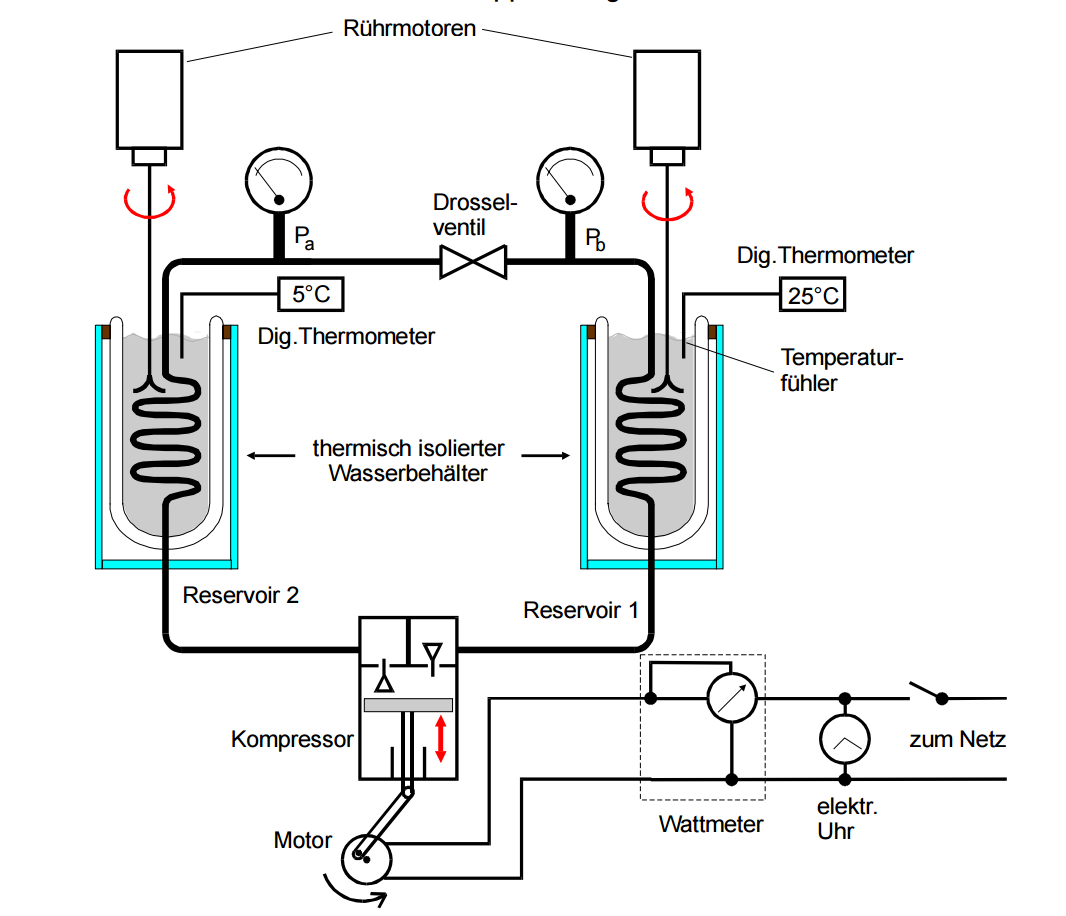
\includegraphics[width=0.99\textwidth]{V2062.png}
  \caption{Der Versuchsaufbau der Messapparatur.}
  \label{fig:V2062}
\end{figure}
In Abbildung \ref{fig:V2062} zu sehen ist der schematische Aufbau der
verwendeten Wärmepumpe. Als Transportmedium zirkuliert angetrieben von einem
Kompressor das Gas Dichloridfluormethan $(Cl_2F_2C)$. Durch das Drosselventil
wird ein Druckunterschied innerhalb der Apparatur erzeugt, sodass in der
Kupferspirale vom zweiten Reservoir das Medium verdampft und dem Wasser dabei die
erforderliche Verdampfungswärme $Q_2$ entzieht. Das Medium wird daraufhin
adiabatisch komprimiert und in die Kupferspirale von Reservoir 1 geleitet.
Dort wird es infolge des höheren Drucks kondensiert und die aufgenommene Wärmemenge
$Q_2+A$ wird abgegeben. Neben zwei Thermometern, die Temperatur messen und 2
Manometern, die den Druck auf beiden Seiten des Kompressors bzw. des
Drosselventils angeben, ist an dem Kompressor noch zusätzlich ein Wattmeter
angeschlossen. Dieses zeigt die elektrische Leistung als Maß für die verrichtete
mechanische Arbeit an. Um eine gleichmäßige Wärmeverteilung innerhalb der
Wasserreservoirs zu gewährleisten werden zwei Rührmotoren verwendet.

\subsection{Versuchsablauf}
\label{sec:versuchsablauf}
Die beiden Reservoirs werden beide mit je 3 Liter Leitungswasser
gleicher Temperatur befüllt. Nachdem man die Wärmepumpe eingeschaltet hat, werden
die Parameter $p_{\mathup{a}}$, $p_{\mathup{b}}$, $T_1$, $T_2$ und $N$ pro Minute
aufgenommen. Der Versuch endet, wenn das erste Reservoir eine Temperatur von
$\SI{50}{\celsius}$ erreicht.

\end{document}
